\documentclass[a4paper]{article}

\usepackage{graphicx}
\usepackage{subfig}
\usepackage{enumitem}

\begin{document}

{
\LARGE
\begin{center}
    \LARGE{%
        Bottleneck identification for constraint relaxation\\[-0.2em]
        in resource-constrained project scheduling
    }\\[0.5em]
    \large{Errata and corrections}\\[2em]
\end{center}
}

\begin{description}
    \item[Figures 1.2, 3.6, and 3.7]
        Removed incorrect resource consumption of Job 9.
        The caption for Figure 3.6 was corrected as follows:
        \begin{quote}
            ...
            We observe that in the relaxed schedule,
            job 9 would require only a small capacity addition on resource 2,
            should it be scheduled in the corresponding time periods.
            Moreover, most of the capacity requirements could be satisfied
            by migrating unused capacities from resource 1.
        \end{quote}

        \vspace{0.5em}
        \centering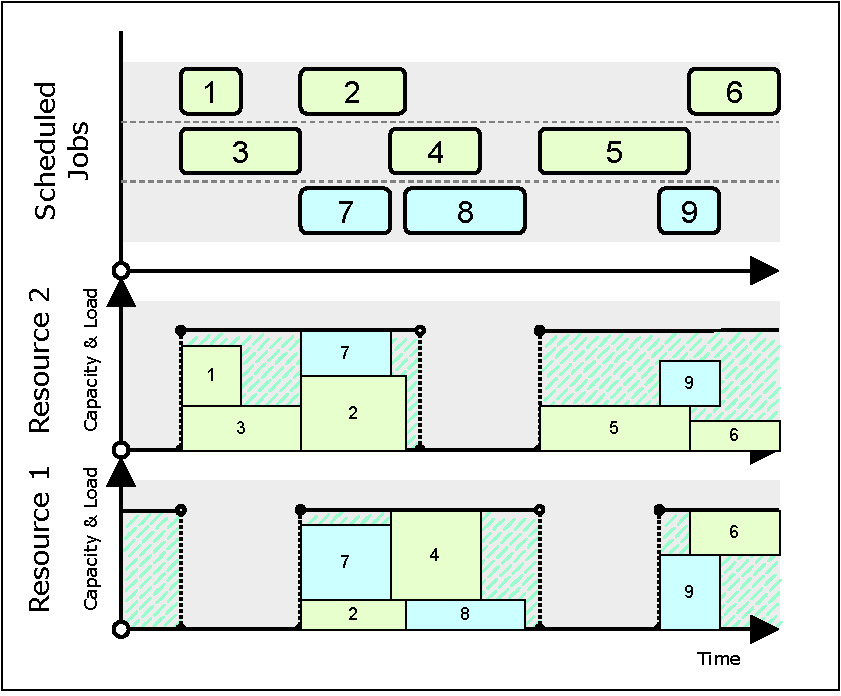
\includegraphics[width=0.45\linewidth]{img/Schedule.pdf}

        {\centering Figure 1.2\\[1em]}

        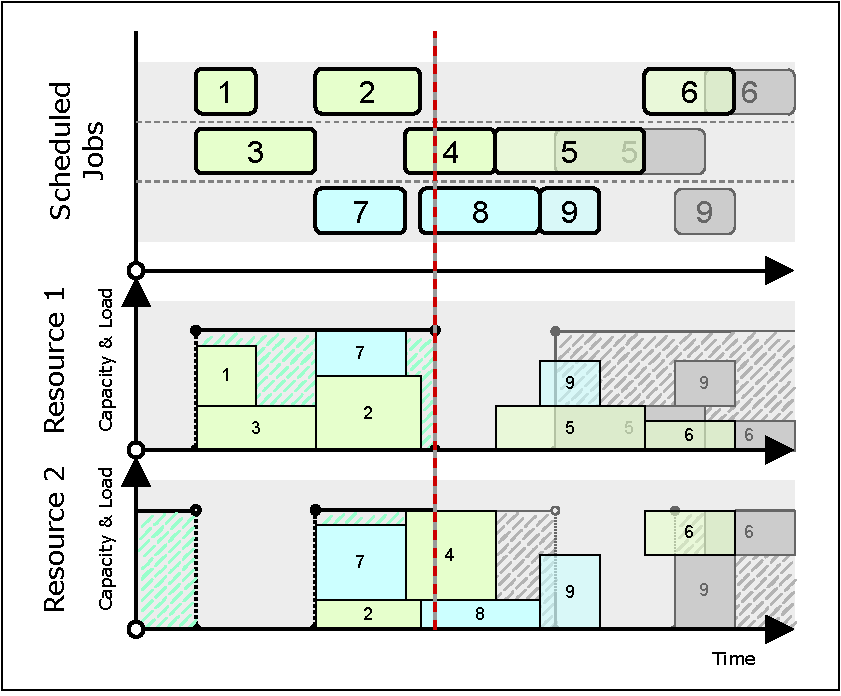
\includegraphics[width=0.45\linewidth]{img/Schedule-Relaxed.pdf}\hfill%
        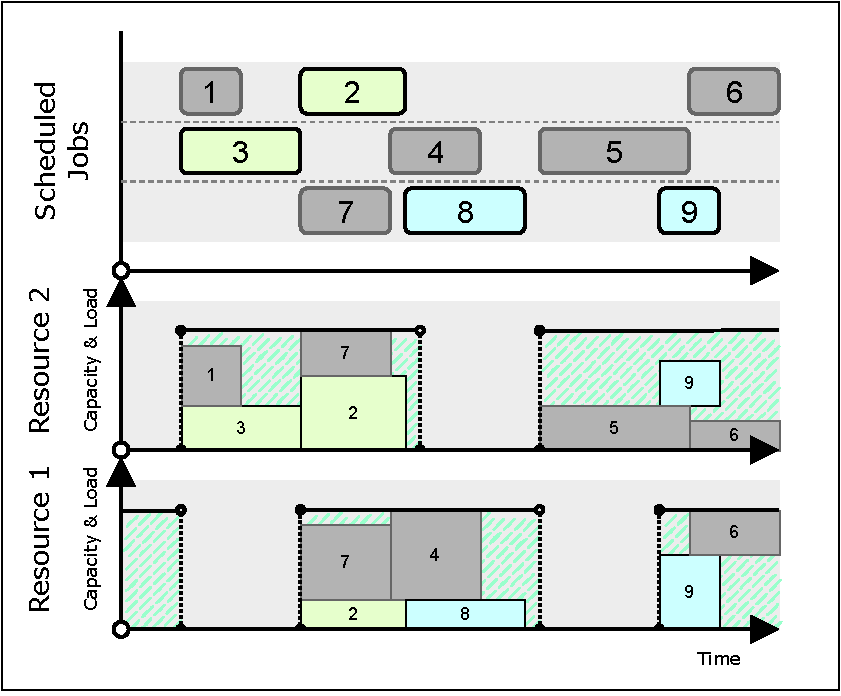
\includegraphics[width=0.45\linewidth]{img/Schedule-Closure.pdf}

        \noindent\makebox[0.45\linewidth]{Figure 3.6}\hfill\makebox[0.45\linewidth]{Figure 3.7}
        
\end{description}

\end{document}
